%!TEX root = ../../thesis.tex
%=============================================================================

\section{Robocup Speech Recognition Test}
In this section, an evaluation of the proposed pipeline in a real work scenario will be presented.
The goal of this evaluation is to evaluate if using the proposed pipeline leads to improved recognition results, in this particular case to increase the accuracy of sound source localization results.
These could be achieved through the result synchronization the proposed pipeline provides.

This evaluation will be based on the Speech \& Person Recognition task of RoboCup@home 2018 \cite{speechrec_2018}, although some minor modifications will be made to the setup.
The evaluation will be conducted on the Pepper robot (TODO cite).

\subsubsection{Software Setup}
Two distinct solutions will be benchmarked:
The existing RoboCup setup and a reimplementation of it within the proposed pipeline.
Both will mainly be comprised of a sound source localization, a speech recognizer and a layer to combine the results of both these components.

\begin{figure}[]
	\centering
	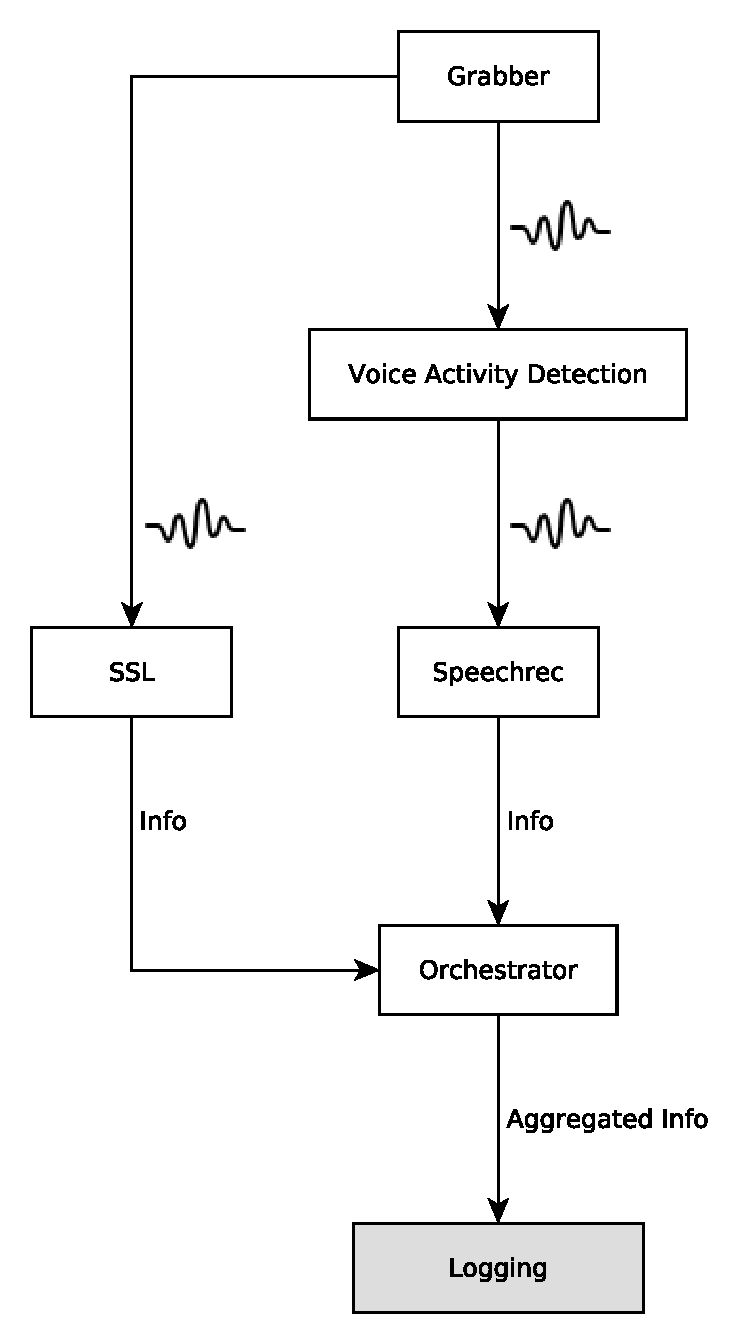
\includegraphics[width=0.66\textwidth]{diagrams/eval_task_proposed.pdf}
	\caption{Setup of of proposed pipeline.
		Audio is only acquired from ALSA at one point, then fed into SSL and speech recognizer separately.
		Generated Information is gathered by the Orchestrator and provided after aggregation to a logging component.}
	\label{pic:eval_task_setup_new}
\end{figure}

The proposed pipeline (see figure \ref{pic:eval_task_setup_new}) will consist mainly of the basic speech recognition setup established as the baseline for the data set evaluation (see chapter \ref{eval:dataset:pipeline:baseline}), i.e. an audio grabber to record audio from a microphone as well as the previously (see chapter \ref{eval:dataset:setup}) established VAD, PocketSphinx speech recognizer and Orchestrator.
As sound source localization a component using pyroomacoustics \cite{pyroomacoustics}, and specifically, its SRP algorithm, will be employed.
Due to the robot providing four channel audio from its four microphones, which are all needed by the SSL, but the speech recognition part of the pipeline requiring only one channel audio, an additional component is needed in the form of a channel splitter.
Since one of the features of the proposed pipeline is synchronization of results, recorded speech recognition results will naturally be enriched with corresponding SSL results.

\begin{figure}[]
	\centering
	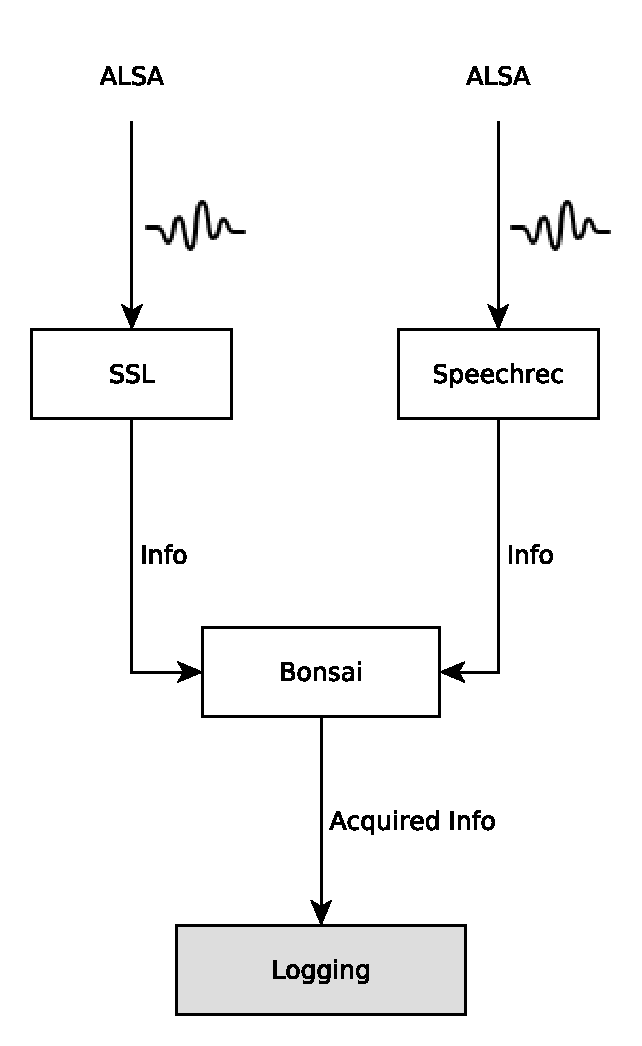
\includegraphics[width=0.5\textwidth]{diagrams/eval_task_old.pdf}
	\caption{Setup of existing solution. 
		Audio is acquired from ALSA by both the speech recognizer and the SSL component independently. 
		Information from both is then collected and combined by Bonsai.
		Bonsai's output is then logged.}
	\label{pic:eval_task_setup_old}
\end{figure}

For the existing solution (see figure \ref{pic:eval_task_setup_old}), the already established PSA will take the role of the speech recognizer.
For sound source localization, a slightly modified variant of the proposed pipelines component will be employed.
To combine both results, a behavior controller called Bonsai \cite{bonsai} will be used.
Bonsai is a TODO.
An channel splitter as with the proposed pipeline is not necessary, as ALSA will assume this task for the PSA.
Since result synchronization is not a feature of primary concern for Bonsai, its default behavior regarding this will be employed, which is to aggregate the SSL results from two seconds to half a second before a speech recognition result was received.

Of course, similar components within both solutions will be equivalently configured.
The output of both solutions will be logged and contain SSL angles and recognized speech.
Both solutions will be run concurrently, to eliminate run-to-run variances between the solutions.
To reduce reciprocal influence, the existing RoboCup setup will run on the robot, while the proposed pipeline will run on a secondary machine, except for the audio grabber node, which must run on the robot.

\subsubsection{Description of the RoboCup@home task}
The RoboCup task would normally start with a small visual person recognition part.
Since visual perception is not part of this thesis, this part of the task will be left out.
The task will instead start with the ''riddles'' game, in which an operator standing in front of the robot will ask the robot five questions which it should answer.

Afterwards, between five and ten persons would surround the robot in the ''blind mans bluff'' game.
Five random persons would then ask the robot each an additional questions.
the robot would turn to the speakers and answer their question.
To ease the evaluation of SSL results, only four persons will partake in the ''blind mans bluff'' game of this evaluation.
One person each will stand directly in front of the robot, behind the robot and to either side of the robot, with circa a 90$^\circ$ shift in angle with respect to the initial orientation of the robot (see figure \ref{pic:eval_task}).
All questions for the task will be generated from the publicly available RoboCup 2018 command generator.



\begin{figure}[]
	\centering
	\subfloat[Scenario for baseline of proposed pipeline]{
		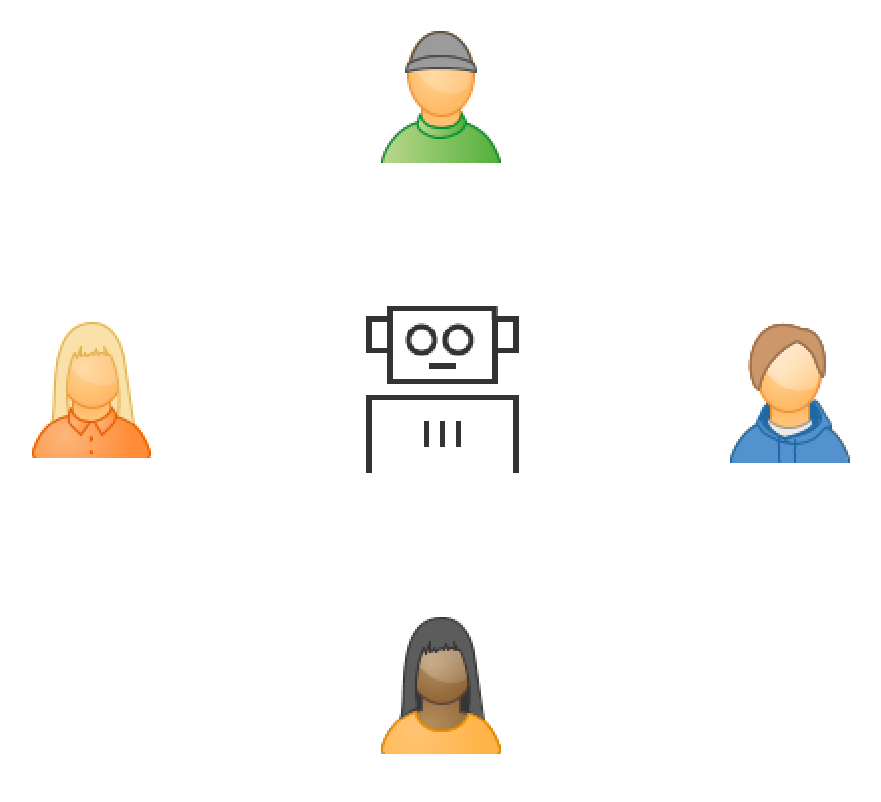
\includegraphics[width=0.5\textwidth]{diagrams/robocup_task_t.pdf}
	}
	\subfloat[Scenario for elongated baseline of proposed pipeline]{
		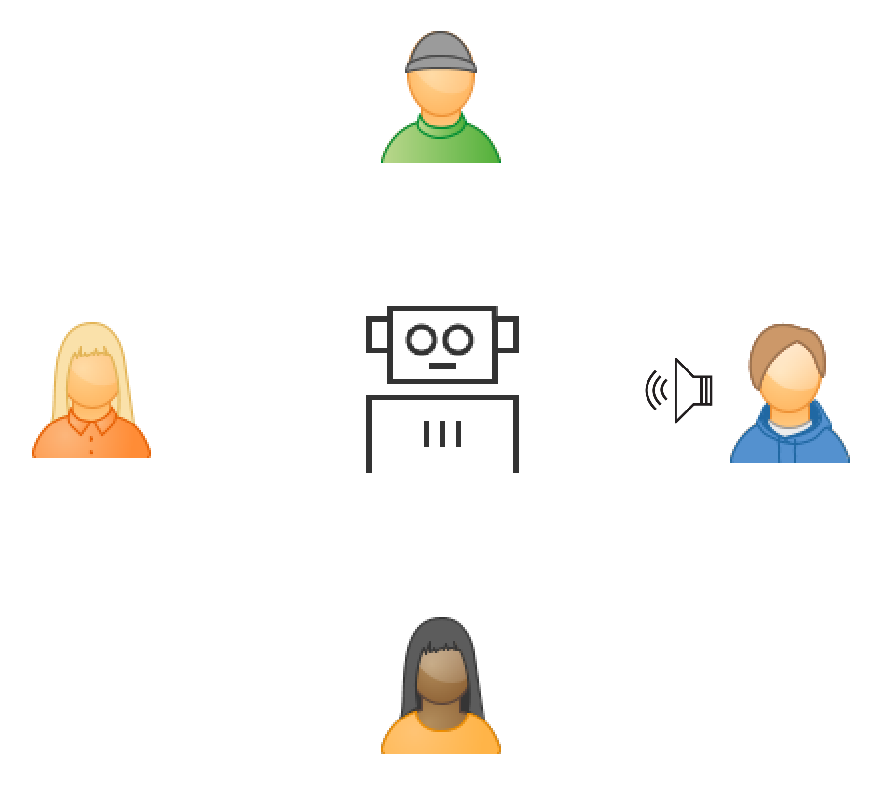
\includegraphics[width=0.5\textwidth]{diagrams/robocup_task_t1.pdf}
	}
	\caption{Test scenario for the RoboCup task}
	\label{pic:eval_task}
\end{figure}

Simultaneous execution of both solutions requires small changes to the task.
Since the robot can not turn to two different angles at once, instead of turning the robot to the speaker, logged angle information was used to evaluate SSL results.
For similar reasons and since producing answers to the questions can be done rather easily, recognizing the correct question was counted as correctly answered.
Both these information can easily be acquired by inspecting the logged output of both solutions.

To ease scoring of the task and provide documentation, the task was recorded by a video camera.
The task was conducted eight times, but two of these runs were excluded from the evaluation, due to camera malfunctions.
The recordings of the included runs were made available through TODO.

To simulate the environment preset on most RoboCup events, which are typically conducted in a crowded convention center and to provide non optimal conditions for the sound source localization, extensive noise was generated in front of the robot by two speakers.
This noise is intended to significantly increase the difficulty of SSL, to provide clearer results.
A still of the video recordings can be seen in figure \ref{pic:eval_task_setup_pepper}.
The two speakers seen in the foreground were playing restaurant noises, which consisted mostly of human chatter.

\begin{figure}[]
	\centering
	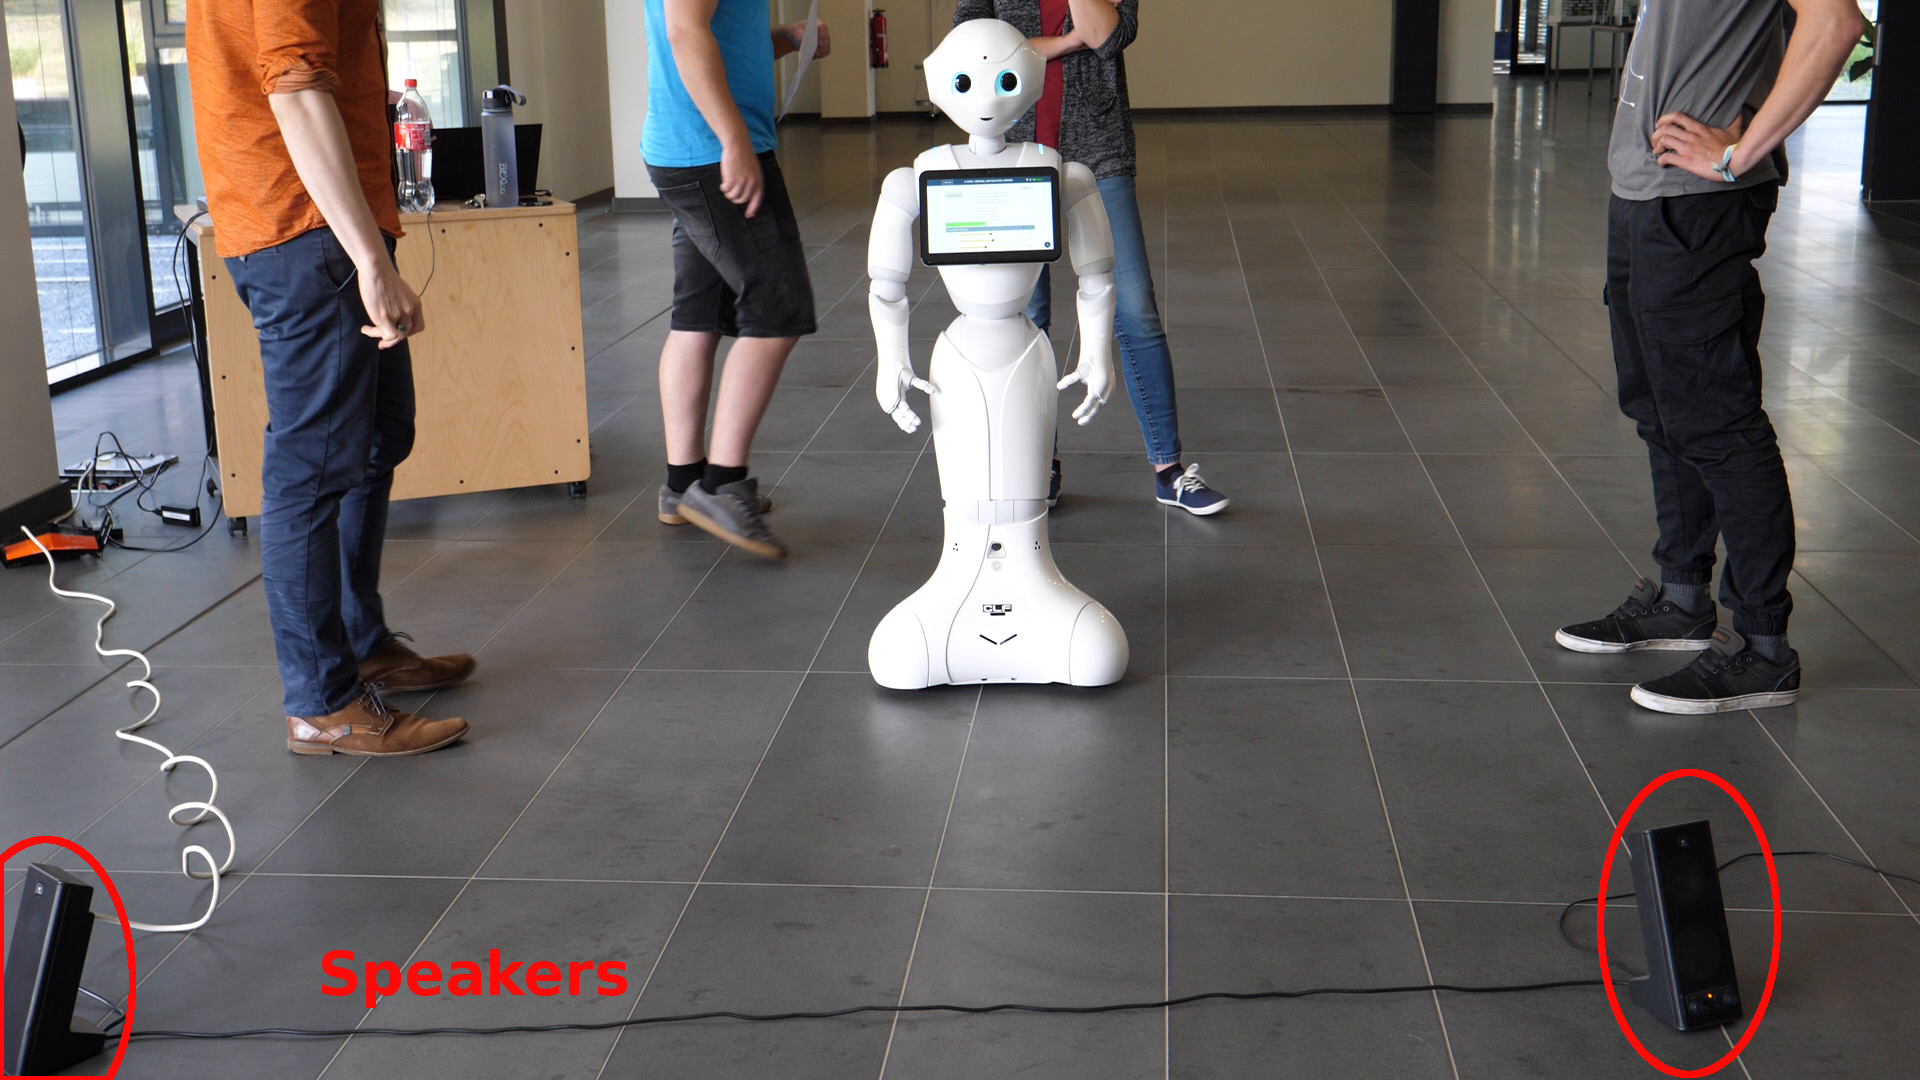
\includegraphics[width=\textwidth]{bilder/eval/pepper_task_setup.png}
	\caption{Evaluation Setup}
	\label{pic:eval_task_setup_pepper}
\end{figure}

\subsubsection{Discussion}
Pinpoint accuracy of SSL results is generally not required.
For the purposes of locating and differentiating speakers from one another, especially in a household environment, where generally only a handful of people are present, any SSL result within a margin of error of +-15$^\circ$ can be regarded as correct.
Rather erroneous detections caused by noise before or after the spoken question should not falsely be included in an analysis on where a speaking person is located.
As such, for the purpose of scoring both pipelines results, any SSL result would be regarded as correct, if it lied inside the proposed 15$^\circ$ margin of error.

Results were manually evaluated by combining information from the recorded videos, spoken questions and logged SSL recordings.
The performance of the existing solution can be seen in figure \ref{table:eval_task_results_old}, while that of the proposed pipeline can be seen in figure \ref{table:eval_task_results_new}.

When comparing results of both solutions, it can easily be seen that similarly to the data set evaluation (see chapter \ref{eval:discussion}), speech recognition results of the proposed pipeline outperform those of the existing solution.
This could be expected, considering that both pipelines use the same speech recognizer as in the data set evaluation.

The SSL results of both solutions may appear quite weak, but one should keep in mind the noise which was specifically generated to increase the difficulty of SSL.
In a real world scenario, similar noise may come from a loud dishwasher or TV.
A robot should however still be able to locate a person giving it commands when confronted by such challenging environments.

The proposed pipeline provided slightly more correct SSL results, which is to say it produced five opposed to the four of the existing solution where 30 were maximally possible.
Both factors in when comparing the actual scores of the RoboCup task, where the proposed pipeline outperforms the existing solution.
However, we consider this score to not be very meaningful, as most of it is caused by the proposed pipelines speech recognizer outperforming the existing solutions one.

Additionally, we generated information about the average error of the SSL results, as we consider these in this particular case to be more significant to the evaluation due to the TODO.
When comparing them, the proposed pipeline outperforms the existing solution in all runs but one, oftentimes by a significant margin.
In run seven and two it (nearly) halves the error.
Overall, the proposed pipeline reduces the error in angle by around 30$^\circ$ in comparison to the existing solution.
We believe this to be the case due to the proposed pipelines enhanced synchronization abilities.
Within the existing solution, shorter questions' SSL results may be random as Bonsai's SSL lookup time frame can completely miss the actual time in which the question was asked.

\begin{figure}[]
	\begin{tabular}{ | l | p{3.5cm}  | r | r | r |}
		\hline
		Run & Correctly recognized sentences & Points & Points by SSL & Avg SSL Error \\ \hline
		1 & 50\% & 45 & 0 & 83.4\\ \hline
		2 & 50\% & 40 & 10 & 92.1\\ \hline
		4 & 35\% & 25 &  0 & 116.0\\ \hline
		5 & 40\% & 30 & 10 & 98.4\\ \hline
		6 & 45\% & 40 & 10 & 97.6\\ \hline
		7 & 60\% & 50 & 10 & 105.2\\ \hhline{|=|=|=|=|=|}
		Avg & 46.7\% & 38.3 & 6.7 & 98.78 \\
		\hline
	\end{tabular}
	\caption{Results of the existing pipeline in the RoboCup task}
	\label{table:eval_task_results_old}
\end{figure}

\begin{figure}[ht]
	\begin{tabular}{ | l | p{3.5cm} | r | r | r |}
		\hline
		Run & Correctly recognized sentences & Points & Points by SSL & Avg SSL Error \\ \hline
		1 & 65\% & 50 &  0 & 86.5\\ \hline
		2 & 55\% & 70 & 20 & 46.6\\ \hline
		4 & 55\% & 35 &  0 & 87.9\\ \hline
		5 & 55\% & 50 & 20 & 54.3\\ \hline
		6 & 60\% & 60 &  0 & 82.3\\ \hline
		7 & 60\% & 60 & 10 & 51.9\\ \hhline{|=|=|=|=|=|}
		Avg & 58.3\% & 54.2 & 8.3 & 68.25\\
		\hline
	\end{tabular}
	\caption{Results of the proposed pipeline in the RoboCup task}
	\label{table:eval_task_results_new}
\end{figure}


